\section{Results}
\subsection{CO emission maps}

\begin{figure*}[htbp]
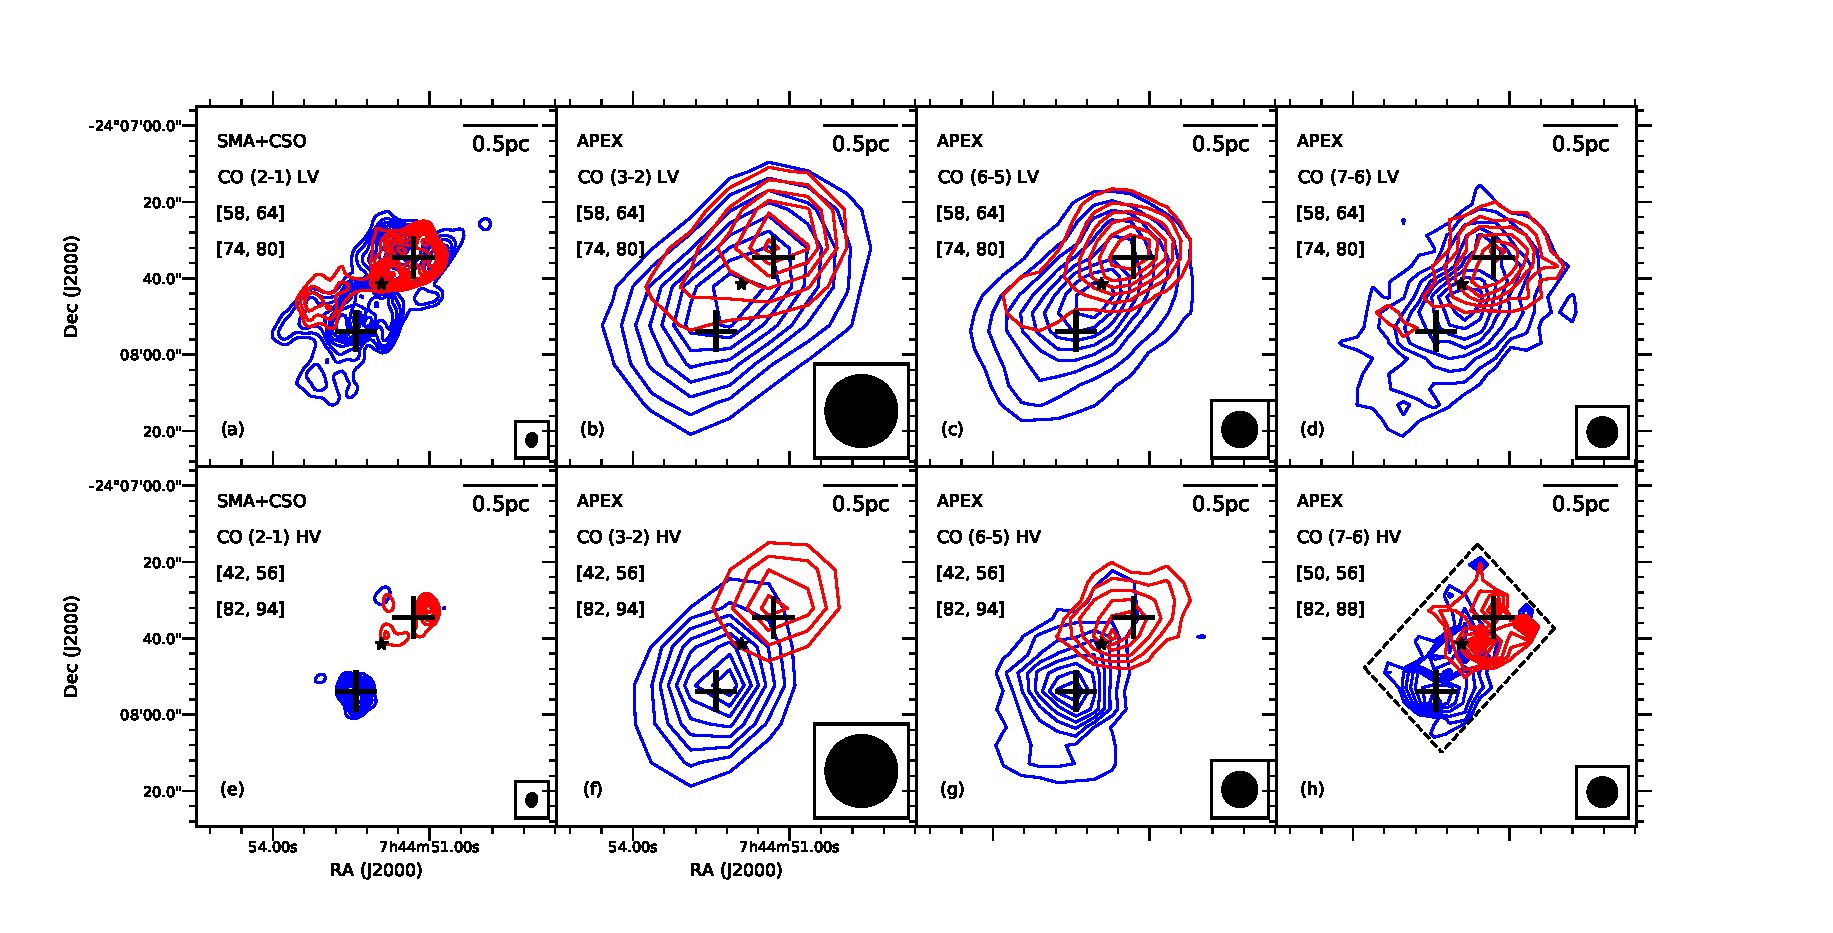
\includegraphics[scale=.65]{./fig/ori_contourall.eps}
\caption{(a)-(d) Low-velocity CO J = (2-1), (3-2), (6-5), (7-6) emissions, integrated from 58 to 64 km s$^{-1} $ for the blueshifted lobe (blue) and from 74 to 80 km s$^{-1}$ for the redshifted lobe (red); (e)-(f) High-velocity CO J = (2-1), (3-2), (6-5) emissions,  integrated from 42 to 56 km s$^{-1} $ for the blueshifted lobe (blue) and from 82 to 94 km s$^{-1}$ for the redshifted lobe (red); (g) High-velocity CO J = (6-5) emission, integrated from 44 to 56 km s$^{-1} $ for the blueshifted lobe (blue) and from 82 to 92 km s$^{-1}$ for the redshifted lobe (red) (h) High-velocity CO J = (7-6) emission, integrated from 46 to 56 km s$^{-1} $ for the blueshifted lobe (blue) and from 82 to 90 km s$^{-1}$ for the redshifted lobe (red). For (a)-(g), the contour levels start from 20\% and continue at steps of 10\% of the peak emission. For (h), the contour levels start from 30\% and continue at steps of 10\% of the peak emission. Edge channels are masked out because of high noise levels. The black star marks the position of a H$_2$O maser spot which is associated with IRAS 07427-2400 \citep{2015PASJ...67...69S}. The beam of each observational dataset is shown in the lower right corner of each panel. \label{fig:figcontour}}
\end{figure*}

The CO (3-2), (6-5) and (7-6) emissions are detected (with fine shapes and with peak intensities greater than 2 $\sigma_{rms}$) in velocity ranges from 42 km s$^{-1}$ to 94 km s$^{-1}$, 44 km s$^{-1}$ to 92 km s$^{-1}$, and 46 km s$^{-1}$ to 90 km s$^{-1}$, respectively. Figure \ref{fig:figcontour} shows the integrated low-velocity (LV) and high-velocity (HV) emissions of the four lines. The velocity ranges chosen to highlight the LV and HV components of the outflowing gas follow those in \citet{2009ApJ...696...66Q}, except that channels with no detections were excluded for the HV component. The morphologies of the bipolar outflow seen in CO (3-2), (6-5) and (7-6) emissions are very similar. Due to the limit of angular resolution, the wide-angle structure highlighted by the CO (2-1) emission is not seen in the CO (3-2), (6-5), (7-6) maps.

\subsection{Physical conditions of the outflow}
\subsubsection{Methodology}

\begin{figure}[tbp]
\plotone{./fig/ratio.eps}
\caption{Ratios of main-beam temperatures of different CO lines at different velocities. Blue symbols denote the measurements from the blueshifted lobe, and red symbols the redshifted lobe. The $V_{\mathrm{outflow}}$ shown here is related to the cloud velocity $v_{\mathrm{cloud}}$ by the relation: $V_{\mathrm{outflow}}$ = $\mid$ $v_{\mathrm{outflow}}$ - $v_{\mathrm{cloud}}\mid$, where $v_{\mathrm{outflow}}$ is the outflow velocity with respect to the local standard of rest. \label{fig:figratio}}
\end{figure}

The physical conditions of the outflow could be constrained by comparing the observed line intensities with results of statistical-equilibrium calculations. To study the four lines at the same spatial resolution, we convolved the CO (2-1), (6-5) and (7-6) maps to the same beam size of the CO (3-2) map. The average rms noises are 0.004 K, 0.04 K and 0.10 K for the convolved CO (2-1), (6-5) and (7-6) data, respectively. We then measured the CO line intensities roughly at the peak positions of the HV components of the two lobes of the convolved CO maps (marked as two crosses in each panel of Figure \ref{fig:figcontour}).  To avoid contaminations from the ambient gas, we limited our analyses to velocity ranges of $\le$ 60 km s$^{-1}$ and $\ge$ 74 km s$^{-1}$. And we focused our analyses on velocities ranges with high signal-to-noise ratios in $\ge$ 46 km s$^{-1}$ and $\le$ 90 km s$^{-1}$. Figure \ref{fig:figratio} shows the observed line-wing ratios of main-beam temperatures ($T_{\mathrm{mb}}$) of different CO lines.  Up to 25 km s$^{-1}$, all line ratios are remarkably constant with velocity. Considering that the $^{13}$CO (2-1) emission was only marginally detected in the outflowing gas with high sensitivity observations\citep{2009ApJ...696...66Q}, we assumed the four $^{12}$CO lines to be optically thin during our analyses. Both the calibration error and the rms noise were taken into account in the belowing analyses.
%(R.A., decl.)$_{J2000}$ = ($07^h44^m52^s.4, -24^d7^m53^s.8$) and (R.A., decl.)$_{J2000}$ = ($07^h44^m51^s.3, -24^d7^m34^s.6$)
%We note that the offsets of the peak positions are within $\sim$ 3$\arcsec$ for different lines at different velocities.
%The uncertainty of the observed intensity mainly consists of two parts: the calibration error and the rms noise. At low velocities, the calibration uncertainty dominates the intensity uncertainty, whereas the rms noise is dominant at high velocities. A combination of the rms noise and the calibration error $\sigma_{obs} = (\sigma_{cal}^2 + \sigma_{rms}^2)^{\frac{1}{2}}$ was used as the observational uncertainty in the belowing analyses.
%errors take into account both the rms noise and the calibration uncertainties.

\subsubsection{Rotation diagram analysis\label{subsec:RD}}

\begin{figure}[tbp]
\plotone{./fig/RD.eps}
\caption{A rotation diagram for CO at 84 km s$^{-1}$.  The fitted line shows the Boltzmann distribution of the rotational populations. The black solid circles show the data with error bars. \label{fig:figrd}}
\end{figure}

Firstly, we performed a simple rotation diagram (RD) analysis \citep{1999ApJ...517..209G} to estimate the excitation conditions of the outflowing gas in each velocity interval under the assumption of local thermal equilibrium (LTE). The population of each level is given by 
\begin{equation}
N_{\mathrm{up}} = \frac{N_\mathrm{CO}}{Z} g_\mathrm{up} e^{-E_\mathrm{up}/kT_\mathrm{kin}},
\end{equation}
where $N_\mathrm{up}$ is the column density in the upper state, $g_\mathrm{up}$ the statistical weight of the upper state, $E_\mathrm{up}$ the upper energy level, $k$ the Boltzmann constant, and $Z$ is the partition function.
The rotation diagram for CO at 84 km s$^{-1}$ is shown in Figure \ref{fig:figrd} as an example. Similar rotation diagrams were found at other velocities. It should be noted that the different energy levels in each velocity bin could be well reproduced with a single-component excitation condition, indicating that the four transitions probe the same volume of gas.  

\subsubsection{Large velocity gradient analysis\label{subsec:LVG}}

\begin{figure*}[!tbp]
\gridline{\fig{./fig/chiimage_nco_paper.eps}{0.5\textwidth}{(a)}
        \fig{./fig/chiimage_nh2_paper.eps}{0.5\textwidth}{(b)}}
 \gridline{\fig{./fig/chiimage_tkin_paper.eps}{0.5\textwidth}{(c)}
      \fig{./fig/chiimage_nh2_low_paper.eps}{0.5\textwidth}{(d)}}
\caption{(a)-(c) The $\chi^2_{\mathrm{red}}$ distribution at 84 km s$^{-1}$ in the [$T$, $n$], [$T$, $N$] and [$n$, $N$] planes, with all other parameters fixed to the values of the best fitting results at this velocity; (d) The $\chi^2_{\mathrm{red}}$ distribution at 84 km s$^{-1}$ in the [$T$, $N$] plane, with the density fixed to the lower limit of density in the 1$\sigma$ confidence region of the fitting result at this velocity. The $\chi^2_{\mathrm{red}}$ of the best fitting result is $\sim$1.00 at 84 km s$^{-1}$. The Solid white contours show the 1$\sigma$ confidence levels. \label{fig:figchi}}
\end{figure*}

Secondly, the non-LTE radiative transfer code RADEX \citep{2007A&A...468..627V} was used to better constrain the gas density ($n_{\mathrm{H}_2}$), the kinetic temperature ($T_{\mathrm{kin}}$) and the CO column density ($N_{\mathrm{CO}}$) of the outflowing gas in each 2 km s$^{-1}$ bin in the Large Velocity Gradient (LVG) approximation. The best fitting results were obtained by minimizing the reduced $\chi^2$ ($\chi^2_{\mathrm{red}}$) between the observed intensities and the model intensities. With four lines observed and three parameters to constrain, our fitting has one degree of freedom. We didn't correct our observed intensities with beam-filling factors. Thus, the derived physical parameters are the average values over the beam.  In Figure \ref{fig:figchi}, the fitting results at 84 km s$^{-1}$ are shown as examples of the $\chi^2_{\mathrm{red}}$ distributions. The $\chi^2_{\mathrm{red}}$ has only one minimum in the [$T$, $N$] plane. The $\chi^2_{\mathrm{red}}$ distribution in the [$T$, $n$] and [$n$, $N$] planes show that the gas is thermalized and no upper limits to the density could be derived, which confirms the LTE assumption of the rotation diagram analysis. Similar $\chi^2_{\mathrm{red}}$ distribution profiles were found at other velocities. The $\chi^2_{\mathrm{red}}$ of the best fitting results varies from 0.10 to 1.72 at different velocities. Though the best-fitted $\chi^2_{\mathrm{red}}$ varies, the $\chi^2_{\mathrm{red}}$ distribution profiles show similarity in morphology at different velocities, indicating that the uncertainties of the fitted parameters may have similar levels at different velocities. So we derive the uncertainties of each parameter of the LVG analysis from the 1$\sigma$ confidence region in the $N$-$T$-$n$ 3-dimensional space at the velocities where $\chi^2_{\mathrm{red}} \sim 1$ as the representative uncertainties of the fitted parameters. The 1$\sigma$ confidence ranges of temperatures are about 40 K - 60 K. The lower limits of gas densities ($n_{\mathrm{lower}}$) are around 10$^5$ cm$^{-3}$, larger than the critical densities of the four lines. The uncertainties of CO column densities are $\sim$ 10 \%. The modeling results predict that the four transitions are optically thin in the outflowing gas, which is consistent with our assumptions. Figure \ref{fig:figsed} shows the comparison of the observed CO intensities with the LVG modeling results in each velocity bin. 

\subsubsection{$T$-$V$ and $N$-$V$ relations}

\begin{figure*}[!tbp]
\gridline{\fig{./fig/tv_paper.eps}{0.5\textwidth}{(a)}
          \fig{./fig/Nv_paper.eps}{0.5\textwidth}{(b)}
          }
\caption{$T$-$V$ and $N$-$V$ diagrams of the G240 outflow, estimated from the rotation diagram analysis (blue x marker for the blue lobe and red x marker for the red lobe) and the LVG analyses (blue open squares for the blue lobe and red open squares for the red lobe). \label{fig:figrelation}}
\end{figure*}

Figure \ref{fig:figrelation} shows the gas temperature and the CO column density of the G240 outflow as functions of the gas velocity, derived from the rotation diagram analysis and the LVG analysis. The $N$-$V$ diagram shows a clear decreasing trend of CO column density with outflow velocity, while the $T$-$V$ diagram shows that the gas temperature has no obvious dependence on gas velocity. We reran the rotation diagram analysis and the LVG analysis on line intensities measured at several different positions, and similar line ratios and modeling results with Figure \ref{fig:figratio} and Figure \ref{fig:figrelation} were found. 
%Thus, we exclude the systematic bias from choices of positions for measuring the line intensities.




